% !TEX program = pdflatex
% !TEX enableSynctex = true
\documentclass[aspectratio=169,10pt]{beamer}

%%%%%%%%%%%%%%%
\usepackage{booktabs}
\usepackage{xspace}
\usepackage{ulem}
\usepackage{subfig}
\usepackage{graphicx}
\usepackage{multirow}
\usepackage[capitalise,noabbrev]{cleveref} 
\usepackage{datatool}
\usepackage{algorithm} 
\usepackage{algpseudocode} 
\usepackage{empheq}
\usepackage[many]{tcolorbox}
\usepackage[capitalise,noabbrev]{cleveref}
\usetheme[progressbar=frametitle,block=fill]{metropolis}

\newcommand{\themename}{\textbf{\textsc{metropolis}}\xspace}
\definecolor{emphcolorval}{rgb}{0.23,0.4,0.7}
\definecolor{highlightcolorval}{rgb}{1,0,0}
% Penn colors
\definecolor{PennRed}{RGB}{149, 0, 26}
\definecolor{PennBlue}{RGB}{1, 37, 110}

\setbeamercolor{frametitle}{bg=PennBlue}
\setbeamercolor{progress bar}{fg=PennBlue}
\setbeamercolor{math text}{fg=PennRed}

\setbeamercolor{block title}{fg=PennBlue}
\setbeamercolor{block body}{fg=PennBlue}

\setbeamercolor{block title example}{fg=PennBlue}
\setbeamercolor{block body example}{fg=PennBlue, bg=yellow}

\setbeamersize{text margin left=5.5pt, text margin right=5.5pt}

\definecolor{cosmiclatte}{rgb}{1.0, 0.99, 0.95}
\setbeamercolor{background canvas}{bg=cosmiclatte}
%\titlegraphic{\hfill\includegraphics[height=0.8cm]{/Users/jesusfv/dropbox/Templates_Slides/penn_fulllogo.pdf}}
\newcommand{\emphcolor}[1]{\textbf{\textcolor{emphcolorval}{#1}}}
%\newcommand{\mathcolor}[1]{{\mathbf{\color{emphcolorval}{#1}}}}
\newcommand{\highlightcolor}[1]{{\textbf{\color{highlightcolorval}{#1}}}}

% \usepackage{natbib}
% \bibliographystyle{ecta}

\crefname{equation}{}{}
\newtheorem{proposition}{Proposition}
\newcommand\bigzero{\makebox(0,0){\text{\huge0}}}
\newcommand{\D}[1][]{\ensuremath{\boldsymbol{\partial}_{#1}}}
\newcommand{\R}{\ensuremath{\mathbb{R}}}
\newcommand{\diff}{\ensuremath{\mathrm{d}}}
\newcommand{\ex}{\ensuremath{\mathrm{ex}}}
\newcommand{\set}[1]{\ensuremath{\left\{{#1}\right\}}}
\newcommand{\indicator}[1]{\ensuremath{\mathds{1}\left\{{#1}\right\}}}
\newcommand{\condexpec}[3][]{\ensuremath{\mathbb{E}_{#1}\left[{#2} \; \middle| \; {#3} \right]}}
\newcommand{\prob}[2][]{\ensuremath{\mathbb{P}_{#1}\left( {#2} \right)}}
\newcommand{\cprob}[2]{\ensuremath{\mathbb{P}\left( {#1}\left| {#2} \right. \right)}}
\newcommand{\condcov}[2]{\ensuremath{\mathrm{cov}\left({#1} \; \middle| \; {#2} \right)}}
\newcommand{\expec}[2][]{\ensuremath{\mathbb{E}_{{#1}}\left[ {#2} \right]}}
\newcommand{\bigO}[1]{\ensuremath{\mathcal{O}(#1)}}
\newcommand{\Xdom}{\mathcal{X}}
\newcommand{\Yrange}{\mathcal{Y}}
\newcommand{\Xtrain}{\mathcal{X}_{\mathrm{train}}}
\newcommand{\Xextr}{\mathcal{X}_{\mathrm{extr}}}
\newcommand{\Xhull}{\mathrm{Hull}(\Xtrain)}
\newcommand{\Xtest}{\mathcal{X}_{\mathrm{test}}}
\newcommand{\Ltest}{\ell_{\mathrm{test}}}
\newcommand{\F}{\mathcal{F}}
\newcommand{\Resid}{\mathcal{R}}
\newcommand{\st}{\textrm{s.t.}\,}

\begin{document}
\title{{\vspace{0.4in}\hspace{0.2in}\textcolor{PennBlue}{How Inductive Bias in Machine Learning Aligns with \\ \hspace*{5 mm}Optimality in Economic Dynamics}}}
\author{\hspace{0.2in}Mahdi Ebrahimi Kahou\inst{1}\and
	James Yu\inst{2}  \and Jesse Perla\inst{2} \and Geoff Pleiss\inst{3,}\inst{4}}
\institute{
	\inst{\hspace{0.2in}1}Bowdoin College, Econ Dept\and
	\inst{\hspace{0.2in}2}University of British Columbia, Vancouver School of Economics \and
	\inst{\hspace{0.2in}3} University of British Columbia, Stats Dept \and 
	\inst{\hspace{0.2in}4} Vector Institute
}

\date{\hspace{0.2in}\today }
\maketitle

\begin{frame}{Motivation}
	\begin{center}
		\emphcolor{In the long run we are all dead---{\it J.M. Keynes, A Tract on Monetary Reform (1923)}}
	\end{center}
	\begin{itemize}
		\item Numerical solutions to dynamical systems are central to many quantitative fields in economics.
		\vspace{0.1in}
		\item Dynamical systems in economics are \emphcolor{boundary value} problems:
		\vspace{0.1in}
		\begin{enumerate}
				\item Boundary is at \emphcolor{infinity}.
				\vspace{0.05in}
				\item The values at the boundary are potentially \emphcolor{unknown}.
				\vspace{0.05in} 
				 condition. 
		\end{enumerate}
		\item Resulting from \emphcolor{forward looking} behavior of agents.
		\vspace{0.1in}
		\item Examples: Transversality  and ``no-bubble" condition.
		\vspace{0.1in}
		\item Without them the problems are ill-posed  and have infinitely many solutions: 
		\vspace{0.1in}
		\begin{itemize}
			\item These forward-looking boundary conditions are the key limitation on increasing dimensionality.
		\end{itemize}
	\end{itemize}
\end{frame}

\begin{frame}{Contribution}
	
\begin{enumerate}
	\item \emphcolor{Inductive bias alignment}:
	\begin{itemize}
		\item The minimum-norm implicit bias of modern ML models automatically satisfies economic boundary conditions at infinity.
	\end{itemize}
	\vspace{0.1in}
	\item \emphcolor{Learning the right set of steady-states}:
	\begin{itemize}
		\item Deep neural networks and kernel machines learn the boundary values, thereby extrapolating very accurately.
	\end{itemize}
	\vspace{0.1in}
	\item \emphcolor{Robustness and speed}:
	\begin{itemize}
		\item Competitive in speed and more stable than traditional methods.
	\end{itemize}
	\vspace{0.1in}
	\item \emphcolor{Consistency of ML estimates}.
\end{enumerate}

\end{frame}


\begin{frame}{Intuition}
	\begin{columns}
		\begin{column}{0.5\textwidth}
			% Content for the left column
			\begin{itemize}
				\item \emphcolor{Minimum-norm implicit bias}: 
				\begin{itemize}
					\item Over-parameterized models (e.g, large neural networks) have more parameters than data points and potentially interpolate the data.
					\vspace{0.05in}
					\item They are biased towards interpolating functions with smallest norm. 
				\end{itemize}
				\vspace{0.1in}
				\item \emphcolor{Violation of economic boundary conditions}:
				\begin{itemize}
					\item Sub-optimal solutions diverge (explode) over time.
					\vspace{0.05in}
					\item They have large or explosive norms.
					\vspace{0.05in}
					\item This is due to the \emphcolor{saddle-path} nature of econ problems.
				\end{itemize}
			\end{itemize}
		\end{column}
		\begin{column}{0.5\textwidth}
		\begin{figure}[t!]
			\centering
			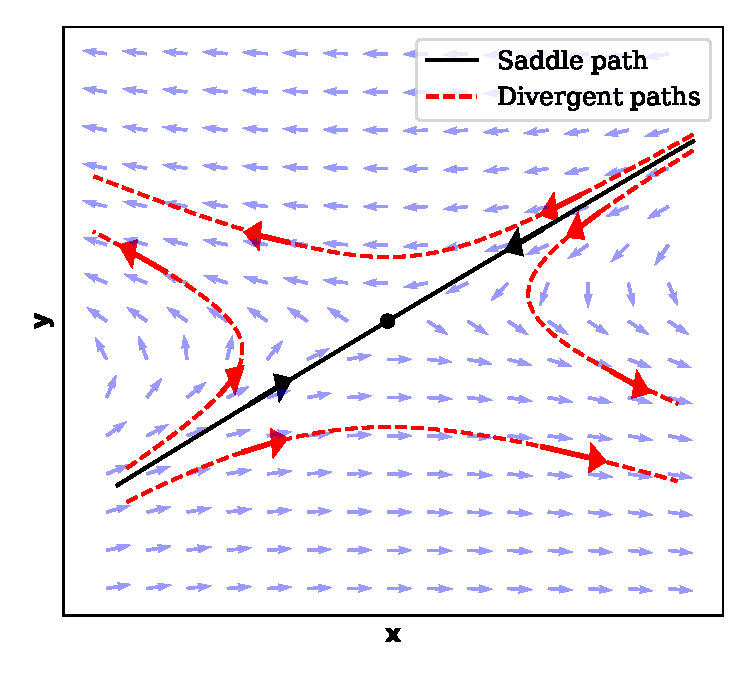
\includegraphics[width=\textwidth]{figs/saddle_path.pdf}
			\vspace{-7mm}
		\end{figure}
		\end{column}
	\end{columns}
\end{frame}

\section{The Problem}

\begin{frame}{The class of problems}
A differential-algebraic system equations, coming from an economic optimization problem:	
	\begin{align}
		\dot{\mathbf{x}}(t) &= \mathbf{F}(\mathbf{x}(t), \mathbf{y}(t))\\ %i.e. law of motions for states, like capital
		\dot{\mathbf{y}}(t) &= \mathbf{G}(\mathbf{x}(t), \mathbf{y}(t))\\
		% coming from the optimizing behaviour, like Euler equations
		\mathbf{0} &= \mathbf{H}(\mathbf{x}(t), \mathbf{y}(t))
		% Usually comes from economics consideratios, like market clearing, no-arbitrage conditions
	\end{align}
$\mathbf{x}\in \mathbb{R}^{N_x}$: state variables, $\mathbf{y}\in\mathbb{R}^{N_y}$: jump variables.
Initial value $\mathbf{x}(0) = \mathbf{x}_0$ and boundary conditions (at infinity)
	\begin{align}
		\mathbf{0} &= \lim_{t\rightarrow\infty} \mathbf{B}(t,\mathbf{x}(t), \mathbf{y}(t))
	\end{align}
\emphcolor{Goal}: finding an approximation for $\mathbf{x}(t)$ and $\mathbf{y}(t)$.\\
	\vspace{0.1in}
\emphcolor{What is the problem?} 
\begin{itemize}
	\item $\mathbf{y}_0$ is unknown. 
	% if y_0 was known I could have solved it a s initial value problem 
	\vspace{0.1in}
	\item The optimal solutions is a \emphcolor{saddle-path}: unstable nature
	\vspace{0.1in}
\end{itemize}
\end{frame}

\section{Method}

\begin{frame}{Method}
	\begin{itemize}
		\item Pick a set of points $\mathcal{D}\equiv \{t_1,\cdots,t_N\}$ for some fixed interval $[0,T]$
		\vspace{0.1in}
		\item Large machine learning models to learn $\hat{\mathbf{x}}(t)$ and $\hat{\mathbf{y}}(t)$
	\begin{align*}
		\min_{\hat{\mathbf{x}}, \hat{\mathbf{y}}} \sum_{t_i \in \mathcal{D}} &\left[\eta_1 \left\Vert \hat{\dot{\mathbf{x}}}(t_i) 
		- \mathbf{F}(\hat{\mathbf{x}}(t_i), \hat{\mathbf{y}}(t_i)(t_i)) \right\Vert_2^2 + \eta_2 \left\Vert \hat{\dot{\mathbf{y}}}(t_i) -  \mathbf{G}(\hat{\mathbf{x}}(t_i), \hat{\mathbf{y}}(t_i)) \right\Vert_2^2\right.\nonumber\\
		&\left.+ \eta_3 \left\Vert \mathbf{H}(\hat{\mathbf{x}}(t_i), \hat{\mathbf{y}}(t_i)) \right\Vert_2^2 + \eta_4 \left\Vert \hat{\mathbf{x}}(0) - \hat{\mathbf{x}}_0 \right\Vert_2^2\right],
	\end{align*}
	\item This optimization \emphcolor{ignores} the boundary conditions.
	 \vspace{0.1in}
	\item The implicit bias automatically satisfy the boundary conditions.
	\vspace{0.1in}
	\item Recent works suggest the implicit bias is toward smallest Sobolev semi-norms.
		\end{itemize}
\end{frame}

\begin{frame}{Ridgeless kernel regression}
\begin{align*}
	\hat{\mathbf{x}}(t) = \mathbf{x}_0+ \int_0^t \hat{\dot{\mathbf{x}}}(\tau) d\tau, &\quad \hat{\mathbf{y}}(t) = \hat{\mathbf{y}}_0+ \int_0^t \ \hat{\dot{\mathbf{y}}}(\tau) d\tau\\
	\hat{\dot{\mathbf{x}}}(t) = \sum_{j=1}^{N} \mathbf{\alpha}^x_j K(t,t_j), &\quad \hat{\dot{\mathbf{y}}}(t) = \sum_{j=1}^{N} \mathbf{\alpha}^y_j K(t,t_j)
\end{align*}
\begin{itemize}
	\item $K(\cdot,\cdot):$ Matérn Kernel, with smoothness parameter $\nu$ and length scale $\ell$.
\end{itemize}
We also solve the ridgeless kernel regression 
	\begin{align*}
	\lim_{\lambda\rightarrow 0} \min_{\hat{\mathbf{x}}, \hat{\mathbf{y}}} \sum_{t_i \in \mathcal{D}} &\left[\eta_1 \left\Vert \hat{\dot{\mathbf{x}}}(t_i) 
	- \mathbf{F}(\hat{\mathbf{x}}(t_i), \hat{\mathbf{y}}(t_i)(t_i)) \right\Vert_2^2 + \eta_2 \left\Vert \hat{\dot{\mathbf{y}}}(t_i) -  \mathbf{G}(\hat{\mathbf{x}}(t_i), \hat{\mathbf{y}}(t_i)) \right\Vert_2^2\right.\nonumber\\
	&\left.+ \eta_3 \left\Vert \mathbf{H}(\hat{\mathbf{x}}(t_i), \hat{\mathbf{y}}(t_i)) \right\Vert_2^2 \right] + \eta_4 \left\Vert \hat{\mathbf{x}}(0) - \hat{\mathbf{x}}_0 \right\Vert_2^2 + \lambda \left[\sum_{m=1}^{N_x}\Vert \hat{\dot{\mathbf{x}}}^{(m)}\Vert^2_{\mathcal{H}}+ \sum_{m=1}^{N_y}\Vert \hat{\dot{\mathbf{y}}}^{(m)}\Vert^2_{\mathcal{H}}\right]
\end{align*}
\end{frame}

\section{Applications}

\begin{frame}{Linear asset pricing}
\begin{align}
	\dot{\mathbf{x}}(t) &= c + g \mathbf{x}(t) \label{eq:asset-pricing-x-dot}\\%:= \mathbf{F}(\mathbf{x}(t), \mathbf{y}(t))
	\dot{\mathbf{y}}(t) &= r \mathbf{y}(t) - \mathbf{x}(t)  \label{eq:asset-pricing-y-dot}\\%:= \mathbf{G}(\mathbf{x}(t), \mathbf{y}(t))
	0 &= \lim_{t\rightarrow \infty} e^{-r t}\mathbf{y}(t) \label{eq:asset-pricing-no-bubble}%:= \mathbf{B}(\mathbf{x}(t), \mathbf{y}(t))
\end{align}

\begin{itemize}
	\item $\mathbf{x}(t)\in \mathbb{R}$: dividends, $\mathbf{y}(t)\in \mathbb{R}$: prices, and $\mathbf{x}_0$ given. 
	\vspace{0.1in}
	\item Equation \cref{eq:asset-pricing-x-dot}: how the dividends evolve in time.
	\vspace{0.1in}
	\item  Equation \cref{eq:asset-pricing-y-dot}: how the prices evolve in time.
	\vspace{0.1in}
	\item Equation \cref{eq:asset-pricing-no-bubble}: ``no-bubble" condition, the boundary condition at infinity. 
	\end{itemize}
\end{frame}

\begin{frame}{Why do we need the boundary condition?}
	\begin{align*}
		\dot{\mathbf{x}}(t) &= c + g \mathbf{x}(t) \\
		\dot{\mathbf{y}}(t) &= r \mathbf{y}(t) - \mathbf{x}(t)
	\end{align*}
	\begin{itemize}
		\item The solutions: 
		\begin{align*}
			\mathbf{y}(t) = \mathbf{y}_f(t) + \zeta e^{rt}
		\end{align*}
		\item $\mathbf{y}_f(t) = \int_0^\infty e^{-r\tau} \mathbf{x}(t+s)ds$: price based on the fundamentals.
		\vspace{0.1in}
		\item $\zeta e^{rt}$: explosive bubble terms, it has to be \emphcolor{ruled out} by the boundary condition.
		%doesnt correspond to any economic variable
		\vspace{0.1in} 
		\item Triangle inequality: $\Vert \mathbf{y}_f\Vert_\mathcal{H} < \Vert \mathbf{y}\Vert_\mathcal{H}$.
		\vspace{0.1in}
		\item The price based on the fundamentals has the \emphcolor{lowest norm}.
	\end{itemize}
\end{frame}

\begin{frame}{Results}
	\begin{figure}[t!]
		\centering
		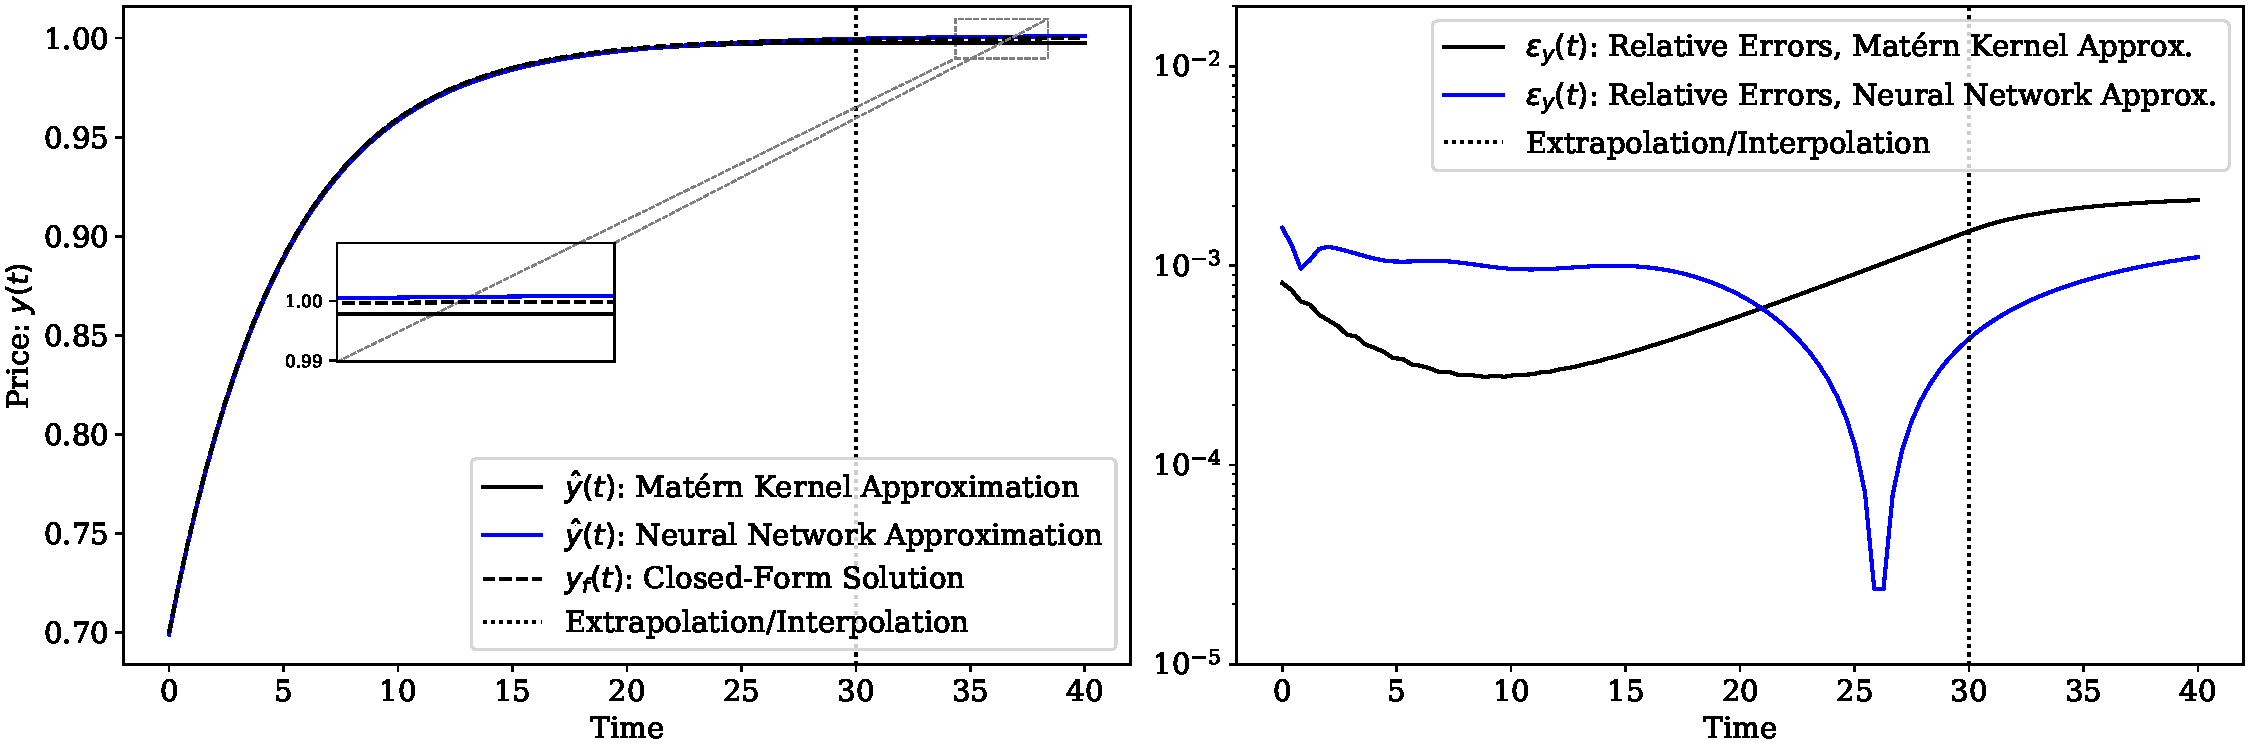
\includegraphics[width=0.8\textwidth]{figs/asset_pricing_contiguous.pdf}
		\caption*{$\mathcal{D} = \{0,1,\cdots,30\}$}
		\vspace{-4mm}
	\end{figure}
	\begin{itemize}
		\item The explosive solutions are ruled out without directly imposing the boundary condition.
		\vspace{0.1in}
		\item Provides a very accurate approximation, both in the short- and medium-run.
		\vspace{0.1in}
		\item Learns the steady-state.
	\end{itemize}
\end{frame}

\begin{frame}{Neoclassical growth model: the agent's problem}
	\begin{align*}
		\max_{\mathbf{y}(t)} &\int_0^\infty e^{-rt}\ln(\mathbf{y}(t))dt\\
		& \text{s.t.} \quad \dot{\mathbf{x}}(t) = f(\mathbf{x}(t)) - \mathbf{y}(t)-\delta \mathbf{x}(t)
	\end{align*}
for a given $\mathbf{x}_0$.


Constructing the Hamiltonian ...
	\begin{align}
		&\dot{\mathbf{x}}(t) = f(\mathbf{x}(t)) - \mathbf{y}(t)-\delta \mathbf{x}(t)\\
		&\dot{\mathbf{y}}(t) = \mathbf{y}(t)\big[f'(\mathbf{x}(t)) -\delta -r\big]\\
		& 0 = \lim_{t\rightarrow \infty} e^{-rt}\frac{\mathbf{x}(t)}{\mathbf{y}(t)}
	\end{align}
	\begin{itemize}
		\item $\mathbf{x}(t)\in \mathbb{R}$: capital and $\mathbf{y}(t)\in \mathbb{R}$: consumption.
		
	\end{itemize}
\end{frame}

\begin{frame}{Why do we need the boundary condition?}
\begin{align*}
	&\dot{\mathbf{x}}(t) = f(\mathbf{x}(t)) - \mathbf{y}(t)-\delta \mathbf{x}(t)\\
	&\dot{\mathbf{y}}(t) = \mathbf{y}(t)\big[f'(\mathbf{x}(t)) -\delta -r\big]
\end{align*}
	\begin{figure}[t!]
		\centering
		\vspace{-4mm}
		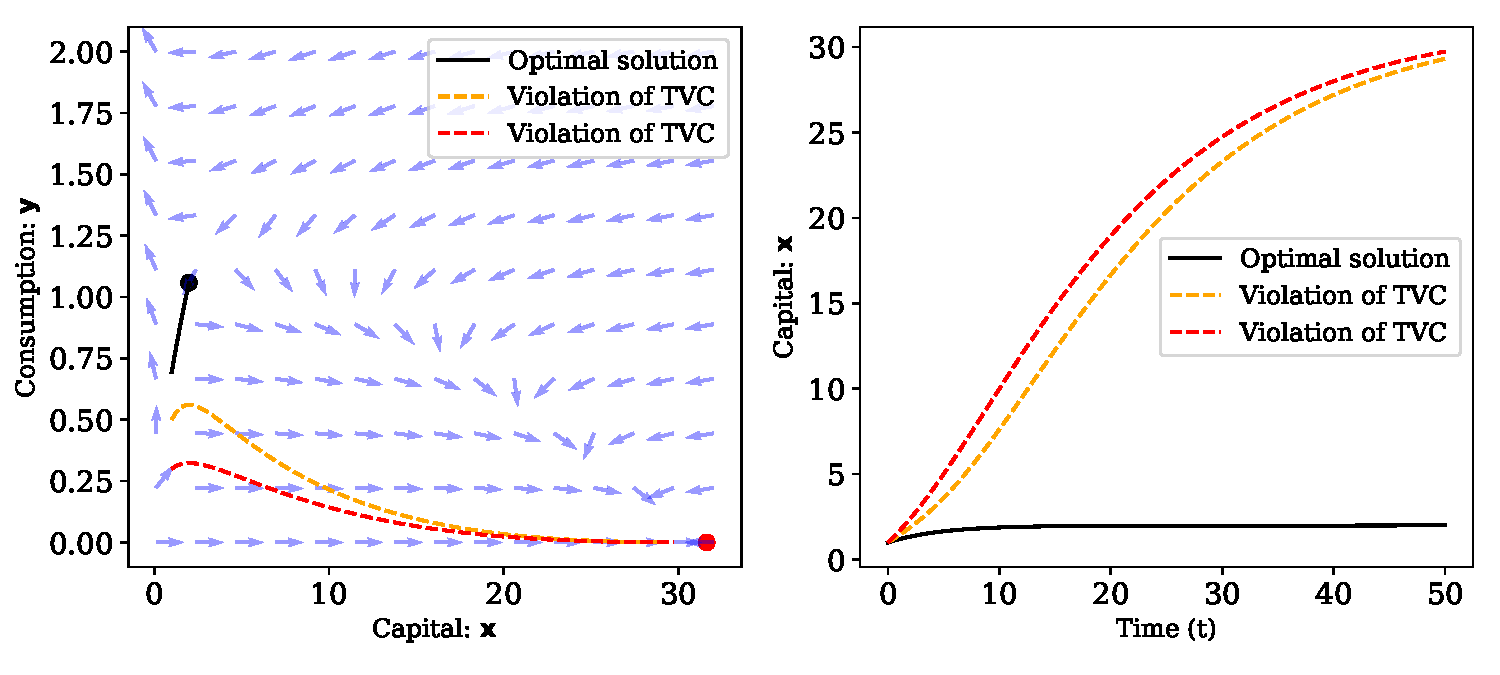
\includegraphics[width=0.8\textwidth]{figs/TVC_violate.pdf}
		\vspace{-4mm}
	\end{figure}
\end{frame}


\begin{frame}{Results}
	\label{ncg:results}
		\begin{figure}[t!]
		\centering
		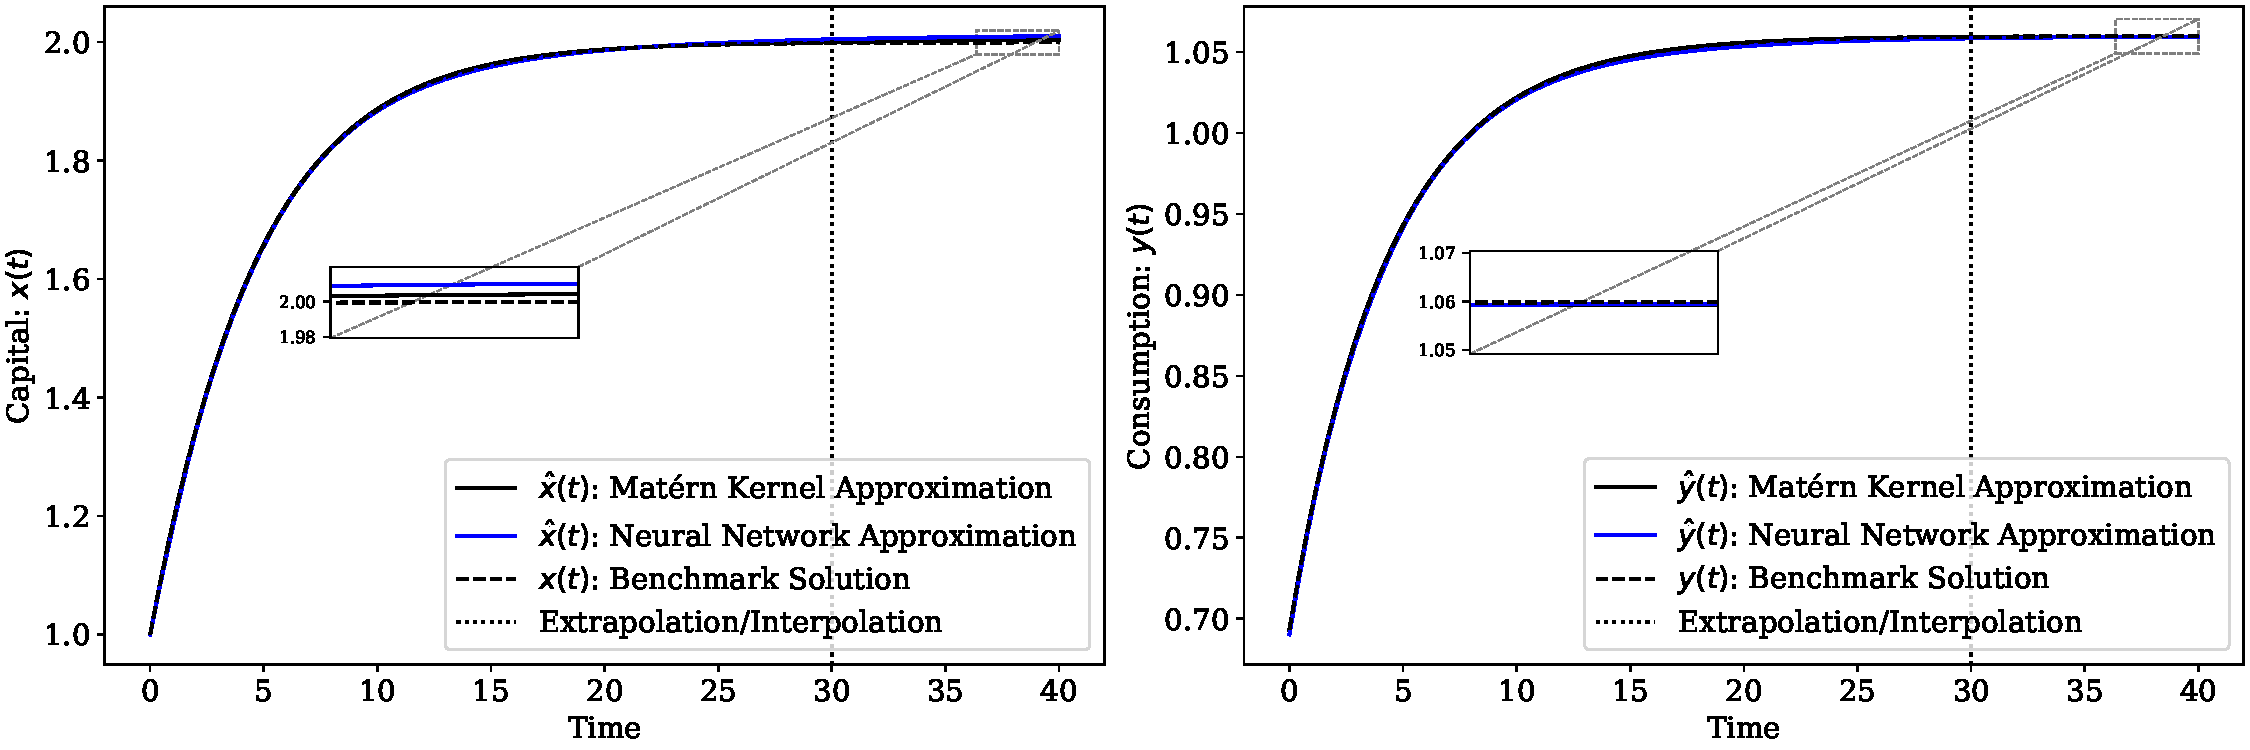
\includegraphics[width=0.8\textwidth]{figs/neoclassical_growth_model_2_by_1.pdf}
		\caption*{$\mathcal{D} = \{0,1,\cdots,30\}$}
		\vspace{-4mm}
	\end{figure}
	\begin{itemize}
		\item The explosive solutions are ruled out without directly imposing the boundary condition.
		\vspace{0.1in}
		\item Provides a very accurate approximation, both in the short- and medium-run.
		\vspace{0.1in}
		\item Learns the  \emphcolor{right steady-state}.
	\end{itemize}
		\hyperlink{errors}{\beamerskipbutton{Relative errors}}
\end{frame}

\begin{frame}{Short time planning: ``In the long run we are all dead" }
	\begin{figure}[t!]
		\centering
		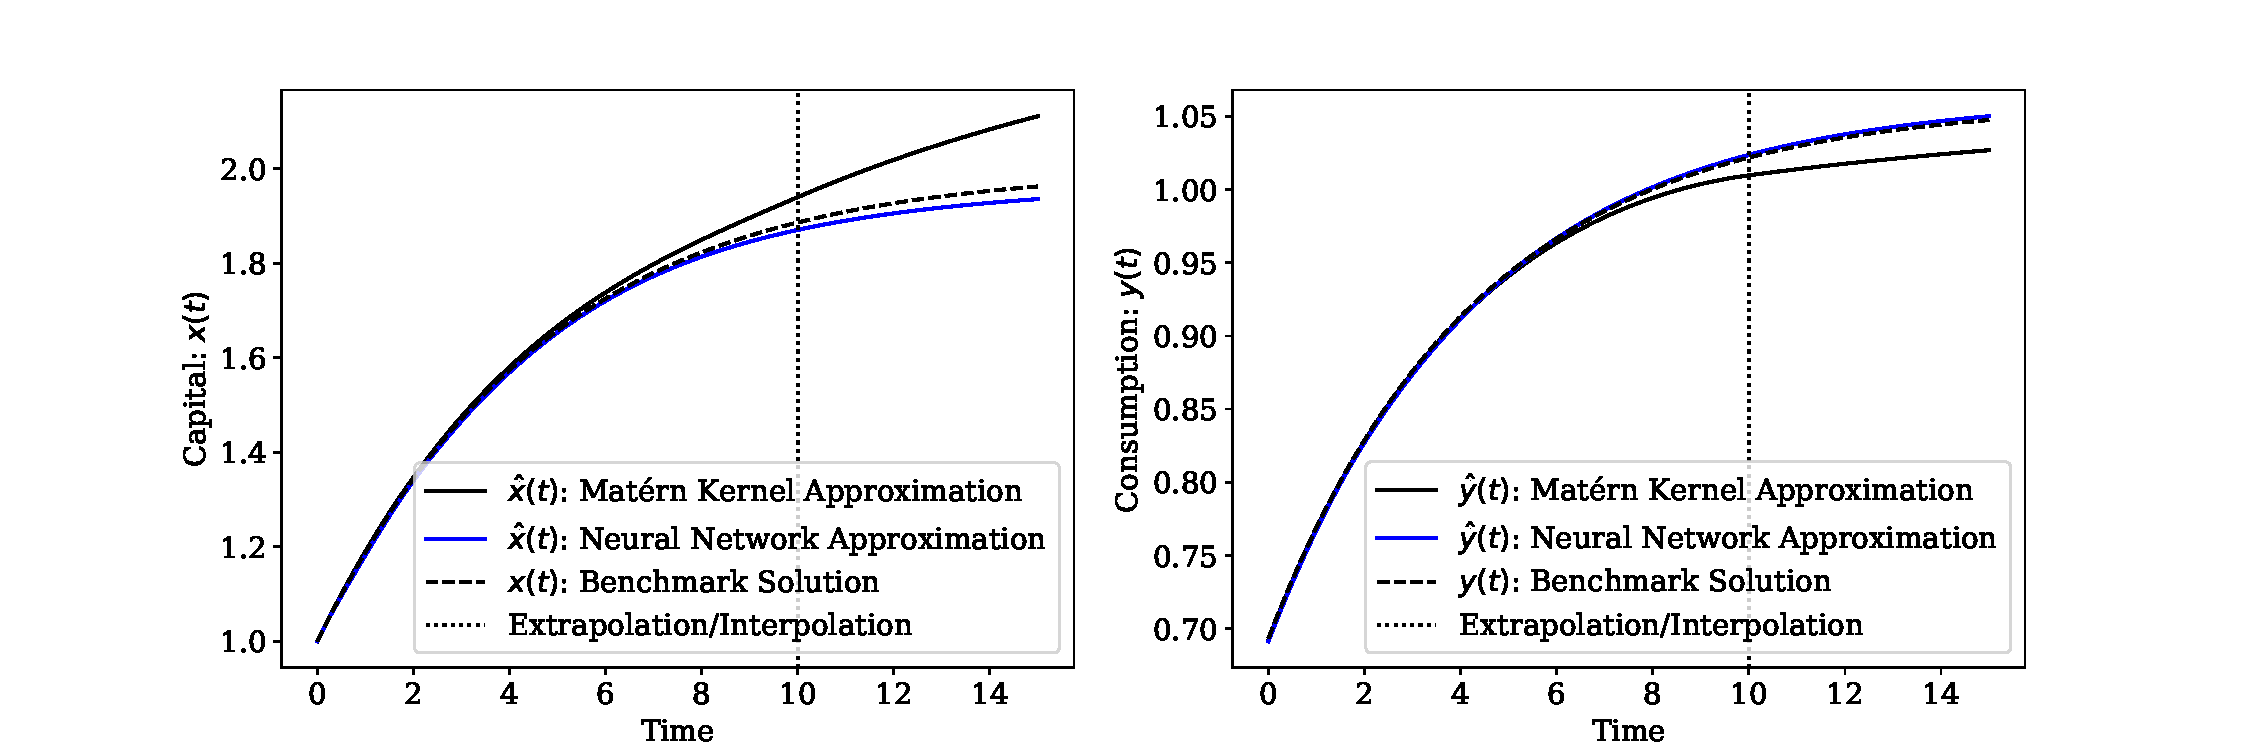
\includegraphics[width=\textwidth]{figs/neoclassical_growth_short_planning.pdf}
		\caption*{$\mathcal{D} = \{0,1,\cdots,10\}$}
		\vspace{-4mm}
	\end{figure}
	\begin{itemize}
		\item The explosive solutions are ruled out without directly imposing the boundary condition.
		\vspace{0.1in}
		\item Provides a very accurate approximation in the short-run.
	\end{itemize}
\end{frame}

\begin{frame}{Neoclassical growth model: concave-convex production function}
	\begin{itemize}
		\item In all examples so far we have had one \emphcolor{saddle-path} converging to a unique \emphcolor{saddle} fixed point.
	\end{itemize}
\end{frame}

\section{Appendix}

\begin{frame}{Neoclassical growth: relative errors}
	\label{errors}
	\begin{figure}[t!]
		\centering
		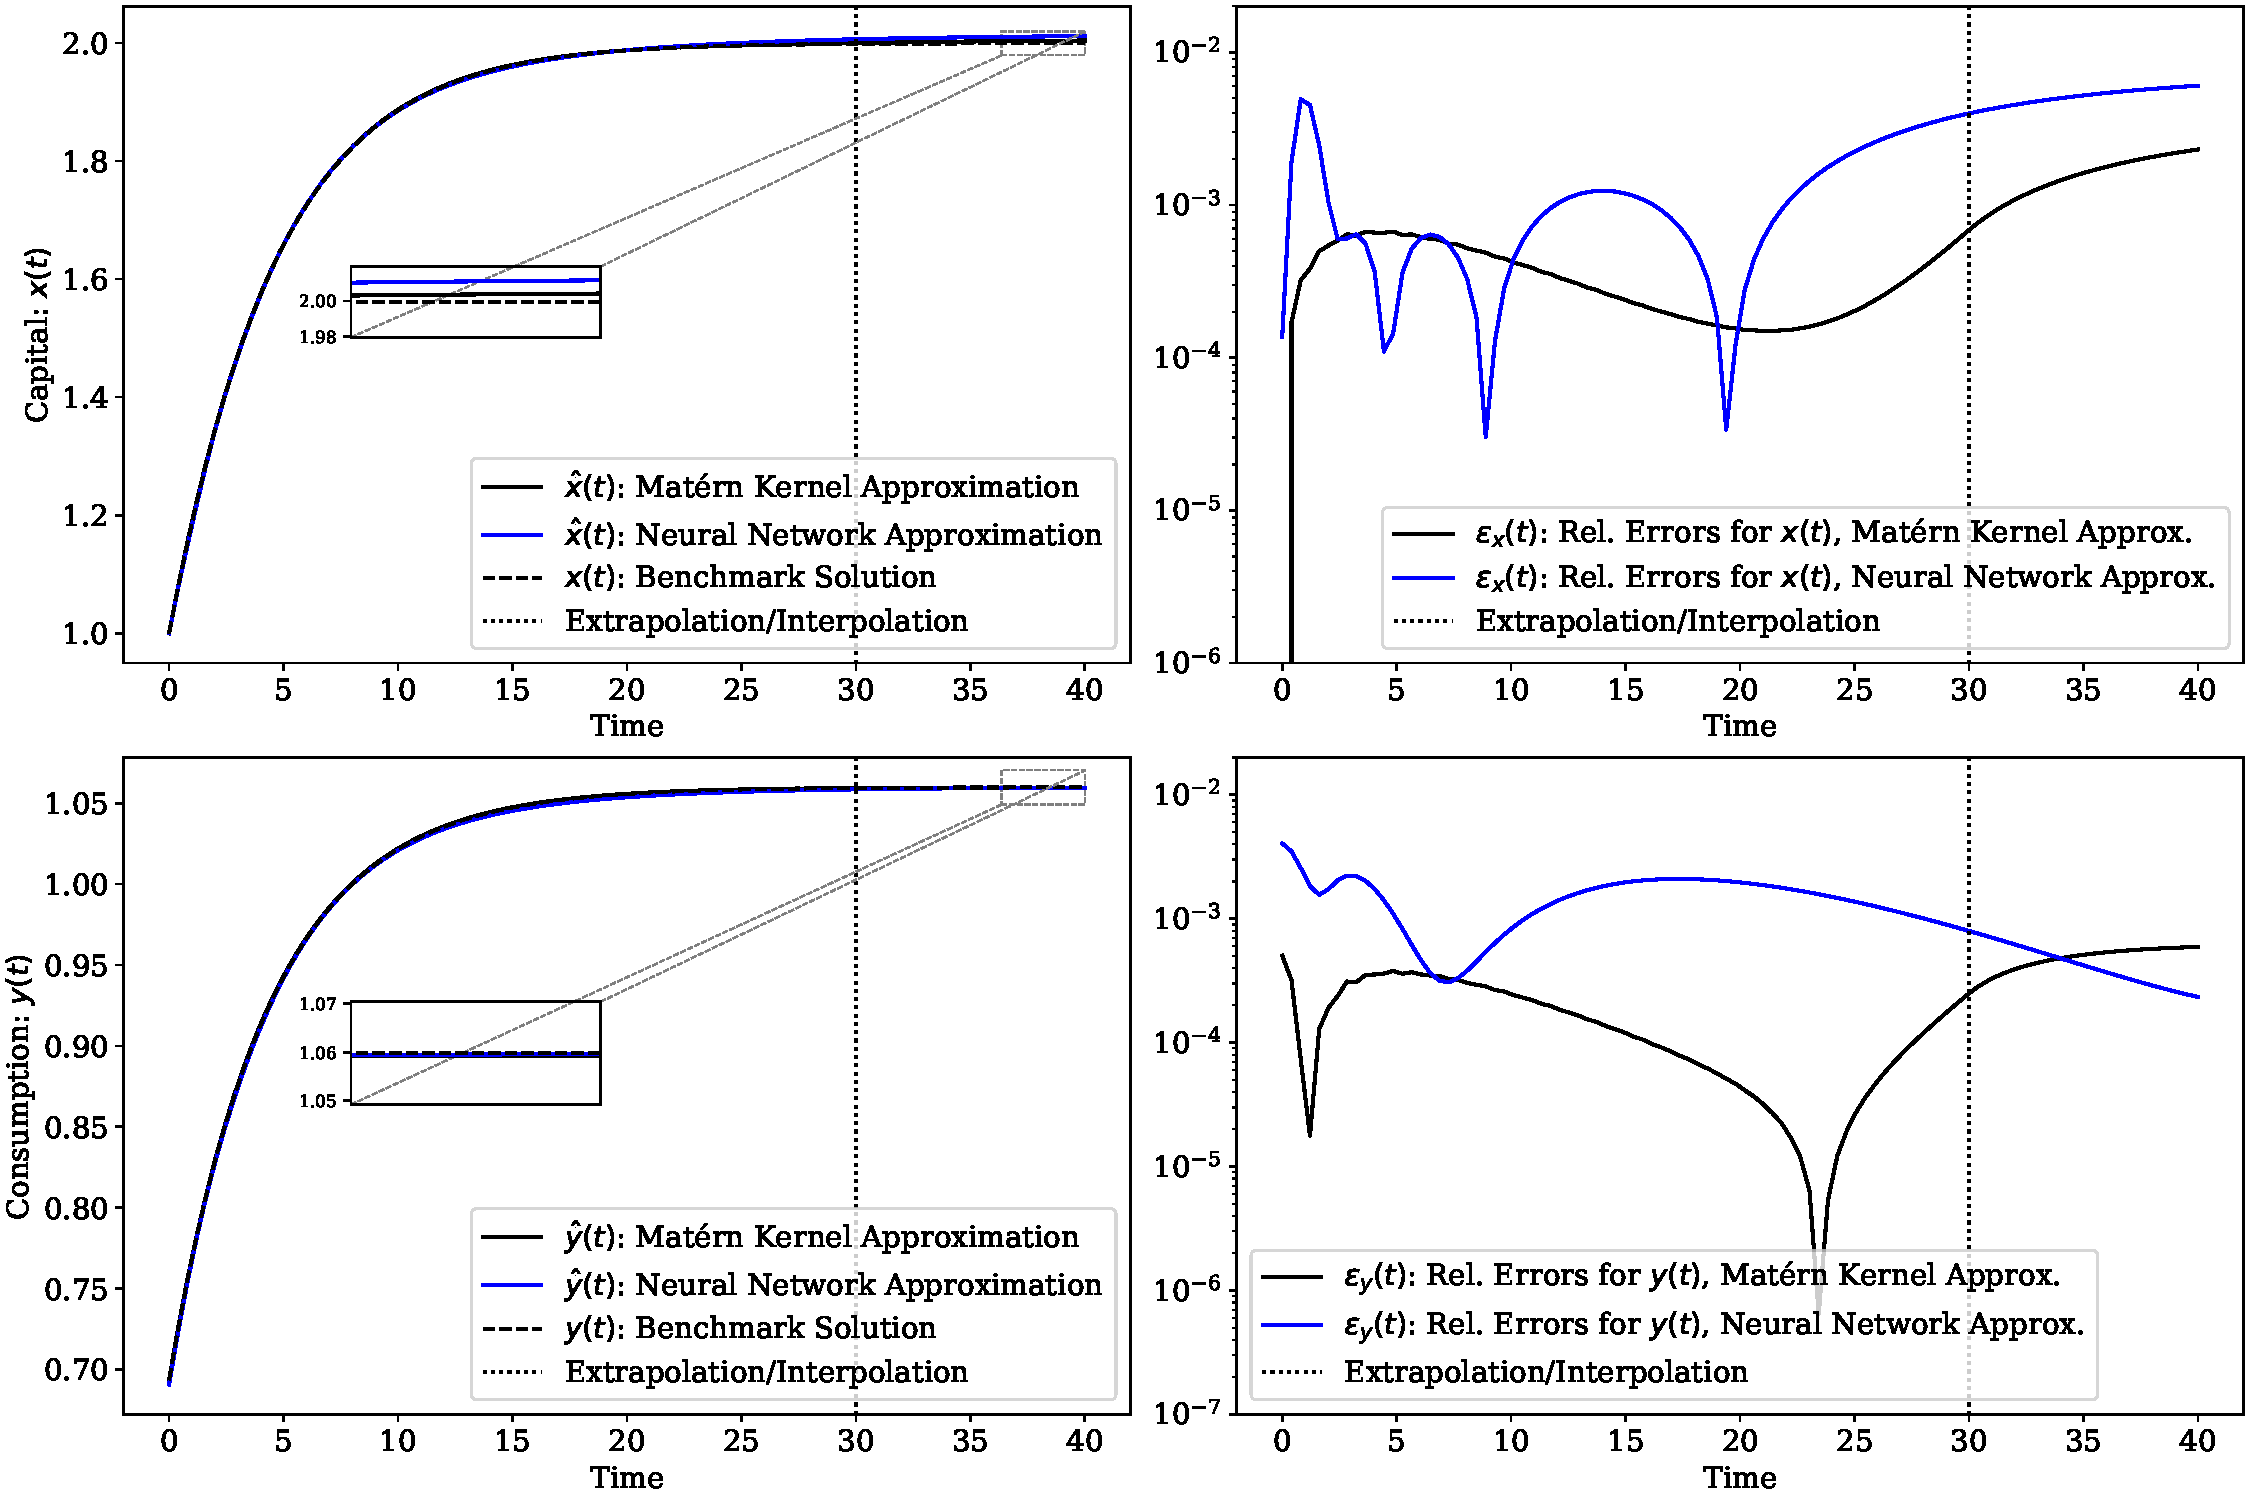
\includegraphics[width=0.7\textwidth]{figs/neoclassical_growth_model_baseline.pdf}
		\vspace{-4mm}
	\end{figure}
			\hyperlink{ncg:results}{\beamerskipbutton{Back}}
\end{frame}

\begin{frame}{contd}
	content...
\end{frame}

\end{document}
